\documentclass[xcolor=dvipsnames]{beamer} 
\usecolortheme[named=OliveGreen]{structure} 
\usetheme[height=7mm]{Rochester} 
\usepackage{tikz}
\usetikzlibrary{arrows,shapes}

\setbeamertemplate{items}[ball] 
\setbeamertemplate{blocks}[rounded][shadow=true] 
\setbeamercovered{invisible}
\setbeamertemplate{navigation symbols}{} % Remove navigation symbols
\setbeamertemplate{headline}{}
\setlength{\parskip}{1em}



\title{Regularized Laplacian Estimation and \\ Fast Eigenvector Approximation}
\author{Patrick~O.~Perry \and Michael~W.~Mahoney}
\institute[NYU Stern and Stanford] {
  NYU Stern \and Stanford University
}
\date{\today}

\begin{document}
% For every picture that defines or uses external nodes, you'll have to
% apply the 'remember picture' style. To avoid some typing, we'll apply
% the style to all pictures.
\tikzstyle{every picture}+=[remember picture]

% By default all math in TikZ nodes are set in inline mode. Change this to
% displaystyle so that we don't get small fractions.
\everymath{\displaystyle}

\begin{frame}
  \titlepage
\end{frame}


\begin{frame}[c]
  \begin{block}{}
  \begin{center}
    \huge{Introduction}
  \end{center}
  \end{block}
\end{frame}


\begin{frame}
  \begin{block}{Eigenvectors reveal structure}
  \begin{description}
    \item[Modularity matrix] community detection
    \item[Graph Laplacian] spectral clustering
    \item[Covariance matrix] factor analysis
  \end{description}
  \end{block}
  
  One way to visualize and simplify high-dimensional data is to form a matrix
  capturing structural information about the dataset and then to focus on
  the leading eigenvectors of this matrix.
\end{frame}


\begin{frame}
  \begin{block}{Diffusions reveal structure}
  \begin{description}
    \item[Heat diffusion] evolution determined by heat equation
    \item[PageRank surfer] random walk with teleportation
    \item[Truncated random walk] finite-length random walk
  \end{description}
  \end{block}

  Alternatively, one can distributed random charge on the data points and
  let the distribution of the charge according to a diffusion; the properties
  of this diffusion are related to the geometry of the dataset.

  Mahoney~and~Orecchia~\cite{MO11-implementing} showed that diffusions arise
  as solutions to \emph{regularized} eigenvector problems.
\end{frame}


\begin{frame}
  \begin{block}{Regularization}
  \begin{description}
    \item[Original problem] minimize $f(x)$
    \item[Regularized problem] minimize $f(x) + \frac{1}{\eta} g(x)$
  \end{description}
  \end{block}

  Regularization is a general principle where we add a penalty function to
  the optimization criterion.  E.g., $g(x) = \|x\|_2$ or $g(x) = \|x\|_1$.
  The solution to the regularized problem is
  often less sensitive to perturbations of the input data, and thus is
  has better statistical robustness.
\end{frame}

\begin{frame}
\centering
{\Large Big picture}
\vspace{-4em}

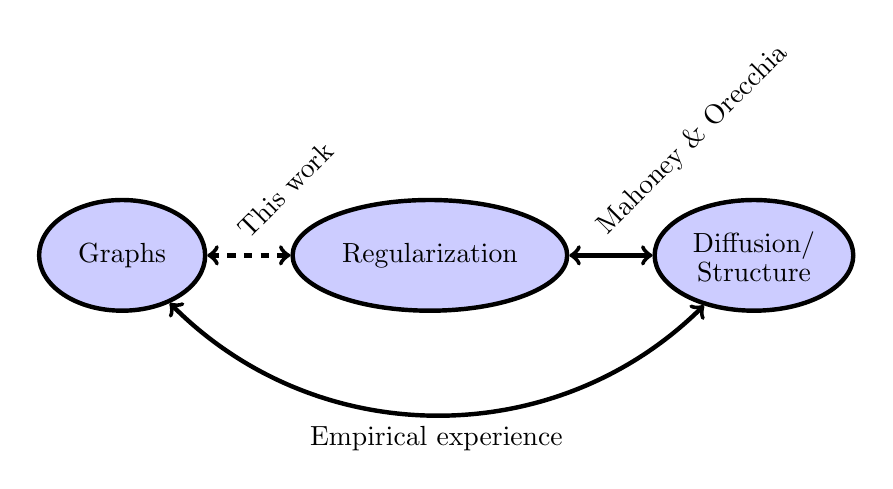
\begin{tikzpicture}[scale=2]
    \matrix[nodes={draw, ultra thick, fill=blue!20, minimum width=6em, minimum height=4em},
        row sep=1em,column sep=3em,ampersand replacement=\&] {
      \node[ellipse] (graphs) {Graphs};\&
      \node[ellipse] (regularization) {Regularization};\&
      \node[ellipse] (structure) {$\stackrel{\hbox{Diffusion/}}{\hbox{Structure}}$};\\
    };
    \path[<->, ultra thick]
      (regularization)
        edge node[auto, rotate=45, anchor=south west] {Mahoney \& Orecchia}
          (structure)
      (graphs)
        edge [bend right=45] node[below] {Empirical experience}
          (structure);
    \path[<->, ultra thick, dashed]
      (graphs)
        edge node[above, rotate=45, anchor=south west] {This work}
          (regularization);
\end{tikzpicture}
From Mahoney and Orecchia, we know that certain regularization penalties
correspond to certain diffusions.
From empirical experience, we know that certain diffusions are more
appropriate for certain classes of graphs.
This current work attempts to complete the circle by showing that certain 
type of regularization make certain implicit assumptions about the graph.
\end{frame}


\begin{frame}
  \frametitle{References}
  \bibliographystyle{unsrt}
  \footnotesize{
    \bibliography{refs}
  }
\end{frame}

\end{document}
